%\iffalse
\let\negmedspace\undefined
\let\negthickspace\undefined
\documentclass[journal,12pt,onecolumn]{IEEEtran}
\usepackage{cite}
\usepackage{amsmath,amssymb,amsfonts,amsthm}
%\usepackage{algorithmic}
\usepackage{graphicx}
\usepackage{textcomp}
\usepackage{array}
\usepackage{xcolor}
\usepackage{txfonts}
\usepackage{listings}
\usepackage{enumitem}
\usepackage{mathtools}
\usepackage{gensymb}
\usepackage[breaklinks=true]{hyperref}
\usepackage{tkz-euclide} % loads  TikZ and tkz-base
\usepackage{listings}
\usepackage{float}
\usepackage{bm}
\usepackage{tikz}
\usetikzlibrary{decorations.markings}



\newtheorem{theorem}{Theorem}[section]
\newtheorem{problem}{Problem}
\newtheorem{proposition}{Proposition}[section]
\newtheorem{lemma}{Lemma}[section]
\newtheorem{corollary}[theorem]{Corollary}
\newtheorem{example}{Example}[section]
\newtheorem{definition}[problem]{Definition}
%\newtheorem{thm}{Theorem}[section] 
%\newtheorem{defn}[thm]{Definition}
%\newtheorem{algorithm}{Algorithm}[section]
%\newtheorem{cor}{Corollary}
\newcommand{\BEQA}{\begin{eqnarray}}
\newcommand{\EEQA}{\end{eqnarray}}
\newcommand{\define}{\stackrel{\triangle}{=}}
\theoremstyle{remark}
\newtheorem{rem}{Remark}
%\bibliographystyle{ieeetr}
\begin{document}
%
\providecommand{\pr}[1]{\ensuremath{\Pr\left(#1\right)}}
\providecommand{\prt}[2]{\ensuremath{p_{#1}^{\left(#2\right)} }}        % own macro for this question
\providecommand{\qfunc}[1]{\ensuremath{Q\left(#1\right)}}
\providecommand{\sbrak}[1]{\ensuremath{{}\left[#1\right]}}
\providecommand{\lsbrak}[1]{\ensuremath{{}\left[#1\right.}}
\providecommand{\rsbrak}[1]{\ensuremath{{}\left.#1\right]}}
\providecommand{\brak}[1]{\ensuremath{\left(#1\right)}}
\providecommand{\lbrak}[1]{\ensuremath{\left(#1\right.}}
\providecommand{\rbrak}[1]{\ensuremath{\left.#1\right)}}
\providecommand{\cbrak}[1]{\ensuremath{\left\{#1\right\}}}
\providecommand{\lcbrak}[1]{\ensuremath{\left\{#1\right.}}
\providecommand{\rcbrak}[1]{\ensuremath{\left.#1\right\}}}
\newcommand{\sgn}{\mathop{\mathrm{sgn}}}
\providecommand{\abs}[1]{\left\vert#1\right\vert}
\providecommand{\res}[1]{\Res\displaylimits_{#1}} 
\providecommand{\norm}[1]{\left\lVert#1\right\rVert}
%\providecommand{\norm}[1]{\lVert#1\rVert}
\providecommand{\mtx}[1]{\mathbf{#1}}
\providecommand{\mean}[1]{E\left[ #1 \right]}
\providecommand{\cond}[2]{#1\middle|#2}
\providecommand{\fourier}{\overset{\mathcal{F}}{ \rightleftharpoons}}
\newenvironment{amatrix}[1]{%
  \left(\begin{array}{@{}*{#1}{c}|c@{}}
}{%
  \end{array}\right)
}
%\providecommand{\hilbert}{\overset{\mathcal{H}}{ \rightleftharpoons}}
%\providecommand{\system}{\overset{\mathcal{H}}{ \longleftrightarrow}}
	%\newcommand{\solution}[2]{\textbf{Solution:}{#1}}
\newcommand{\solution}{\noindent \textbf{Solution: }}
\newcommand{\cosec}{\,\text{cosec}\,}
\providecommand{\dec}[2]{\ensuremath{\overset{#1}{\underset{#2}{\gtrless}}}}
\newcommand{\myvec}[1]{\ensuremath{\begin{pmatrix}#1\end{pmatrix}}}
\newcommand{\mydet}[1]{\ensuremath{\begin{vmatrix}#1\end{vmatrix}}}
\newcommand{\myaugvec}[2]{\ensuremath{\begin{amatrix}{#1}#2\end{amatrix}}}
\providecommand{\rank}{\text{rank}}
\providecommand{\pr}[1]{\ensuremath{\Pr\left(#1\right)}}
\providecommand{\qfunc}[1]{\ensuremath{Q\left(#1\right)}}
	\newcommand*{\permcomb}[4][0mu]{{{}^{#3}\mkern#1#2_{#4}}}
\newcommand*{\perm}[1][-3mu]{\permcomb[#1]{P}}
\newcommand*{\comb}[1][-1mu]{\permcomb[#1]{C}}
\providecommand{\qfunc}[1]{\ensuremath{Q\left(#1\right)}}
\providecommand{\gauss}[2]{\mathcal{N}\ensuremath{\left(#1,#2\right)}}
\providecommand{\diff}[2]{\ensuremath{\frac{d{#1}}{d{#2}}}}
\providecommand{\myceil}[1]{\left \lceil #1 \right \rceil }
\newcommand\figref{Fig.~\ref}
\newcommand\tabref{Table~\ref}
\newcommand{\sinc}{\,\text{sinc}\,}
\newcommand{\rect}{\,\text{rect}\,}
%%
%	%\newcommand{\solution}[2]{\textbf{Solution:}{#1}}
%\newcommand{\solution}{\noindent \textbf{Solution: }}
%\newcommand{\cosec}{\,\text{cosec}\,}
%\numberwithin{equation}{section}
%\numberwithin{equation}{subsection}
%\numberwithin{problem}{section}
%\numberwithin{definition}{section}
%\makeatletter
%\@addtoreset{figure}{problem}
%\makeatother

%\let\StandardTheFigure\thefigure
\let\vec\mathbf

\bibliographystyle{IEEEtran}





\bigskip

%\renewcommand{\thefigure}{\theenumi}
%\renewcommand{\thetable}{\theenumi}
%\renewcommand{\theequation}{\theenumi}

Q: The Fourier cosine series of a function is given by: $f(x) = \sum_{n=0}^{\infty} f_{n}\cos{nx}$. For $f(x) = \cos^{4}x$, the numerical value of $(f_{4} + f_{5})$ is
 
\solution
\begin{table}[h]
\centering
\begin{tabular}{|c|c|c|c|}
        \hline
        \textbf{Parameter} & \textbf{Value(a)} & \textbf{Value(b)} & \textbf{Description}\\
        \hline
	Radius(r) & $3\text{cm}$ & $2\text{m}$ & Radius of each circle \\
        \hline
	Time Period(T) & $2\text{s}$ & $4\text{s}$ & Time period \\
	\hline
	Sense & clockwise & anti-clockwise & Indicated by arrow\\
	\hline
	Initial Phase$(\phi)$ & $\frac{\pi}{2}$ & $\pi$ & Initial angle with x-axis\\
	\hline
\end{tabular}
\caption{Input parameters table}
\label{tab:11.14.11}

\end{table}
\begin{align}
f(x) = &\frac{1}{2}a_0 + a_1 \cos(x) + a_2 \cos(2x) + a_3 \cos(3x) + \ldots \\
&+ b_1 \sin(x) + b_2 \sin(2x) + b_3 \sin(3x) + \ldots \\
\int_{-\pi}^{\pi} f(x)\cos(nx), dx &= \frac{1}{2}a_0 \int_{-\pi}^{\pi} \cos(nx),dx + a_1\int_{-\pi}^{\pi} \cos(x)\cos(nx),dx + a_2\int_{-\pi}^{\pi} \cos(2x)\cos(nx),dx + \ldots \\
&+  b_1\int_{-\pi}^{\pi} \sin(x)\cos(nx),dx + b_2\int_{-\pi}^{\pi} \sin(2x)\cos(nx),dx + \ldots \\
\int_{-\pi}^{\pi} \sin(mx)\cos(nx) ,dx &= 0 \\
\int_{-\pi}^{\pi} \sin(mx)\sin(nx) ,dx &= 
\begin{cases}
    \pi \quad \text{if} \quad m=n \neq 0 \\
    0 \quad \text{otherwise} \\
\end{cases} \\
\int_{-\pi}^{\pi} \cos(mx)\cos(nx) ,dx &=
\begin{cases}
    2\pi \quad \text{if} \quad m=n=0 \\
    \pi \quad \text{if} \quad m=n\neq0 \\
    0 \quad \text{if} \quad m \neq n \\
\end{cases} \\
    \therefore f_n &= \frac{1}{\pi}\int_{-\pi}^{\pi} f(x)\cos{nx} \,dx \\
f_4 &= \frac{2}{\pi} \int_{0}^{\pi} (\cos x)^4 \cos(4x) \, dx \\
&= \frac{2}{\pi} \left( \frac{3}{8} \int_{0}^{\pi} \cos(4x) \, dx + \frac{1}{2} \int_{0}^{\pi} \cos(2x) \cos(4x) \, dx + \frac{1}{8} \int_{0}^{\pi} \cos(4x)^2 \, dx \right) \\
&= \frac{2}{\pi} \left( \frac{3}{8} \frac{1}{4} \sin(4x) \Bigg|_{0}^{\pi} + \frac{1}{2} \left[\frac{1}{6} \sin(6x) + \frac{1}{2}\sin(2x) \right] \Bigg|_{0}^{\pi} + \frac{1}{8} \frac{1}{2} \left[ x + \frac{1}{8} \sin(8x) \right] \Bigg|_{0}^{\pi}  \right) \\
&=\frac{1}{8} \\
f_5 &= \frac{2}{\pi} \int_{0}^{\pi} (\cos x)^4 \cos(5x) \, dx \\
&= \frac{2}{\pi} \left( \frac{3}{8} \int_{0}^{\pi} \cos(5x) \, dx + \frac{1}{2} \int_{0}^{\pi} \cos(2x) \cos(5x) \, dx + \frac{1}{8} \int_{0}^{\pi} \cos(4x) \cos(5x) \, dx \right) \\
&= \frac{2}{\pi} \left(\frac{3}{8} \frac{1}{5} \sin(5x) \Bigg|_{0}^{\pi} + \frac{1}{2} \left[ \frac{1}{7} \sin(7x) + \frac{1}{3} \sin(3x) \right] \Bigg|_{0}^{\pi} + \frac{1}{2} \left[ \frac{1}{9} \sin(9x) + \sin(x) \right] \Bigg|_{0}^{\pi} \right) \\
&= 0 \\
\therefore f_4+f_5 &= 0.125
\end{align}
\begin{figure}[ht]
	\centering
	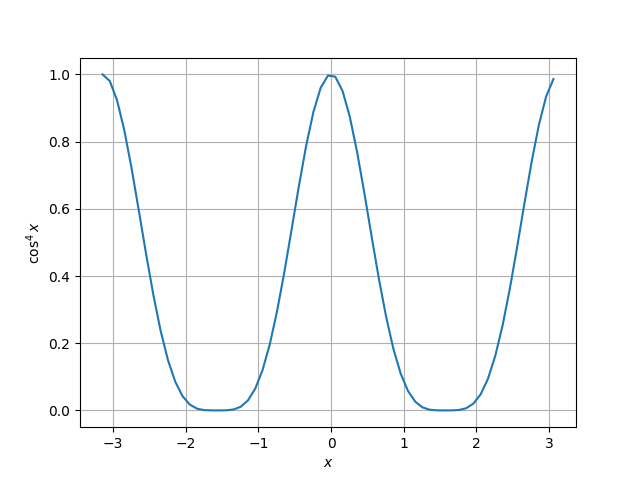
\includegraphics[width=0.8\textwidth]{./figs/fig1.png}
\end{figure}
\end{document}
